\subsection{A Computer Map}

This section maps out a computer using the Intel architecture at three zoom
levels: the motherboard, the CPU, and the execution core, focusing on the
concepts needed to understand SGX and analyze its security properties. Most
details in here are documented in Intel's
\textit{Optimization Reference Manual} \cite{intel2014optimization}.


\subsubsection{The Motherboard}
\label{sec:motherboard}

A computer's components are connected by a printed circuit board called a
\textit{motherboard}, which consists of \textit{sockets} connected by
\textit{buses}. Sockets connect chip-carrying \textit{packages} to the board.
The Intel documentation uses the term ``package'' to specifically refer to a
CPU.

Figure~\ref{fig:motherboard} shows the most relevant chips, from an SGX
perspective. The CPU's package (described in \S~\ref{sec:cpu_die}) is the only
piece of trusted hardware in the SGX model. The \textit{Platform Controller
Hub} (PCH) houses (relatively) low-speed I/O controllers driving the slower
buses in the system, like SATA, used by storage devices, and USB, used by
input peripherals. Motherboards also have a flash memory chip that hosts
firmware which implements the \textit{Unified Extensible Firmware Interface}
(UEFI). The firmware contains the boot code and the SMM handler.

\begin{figure}[hbt]
  \center{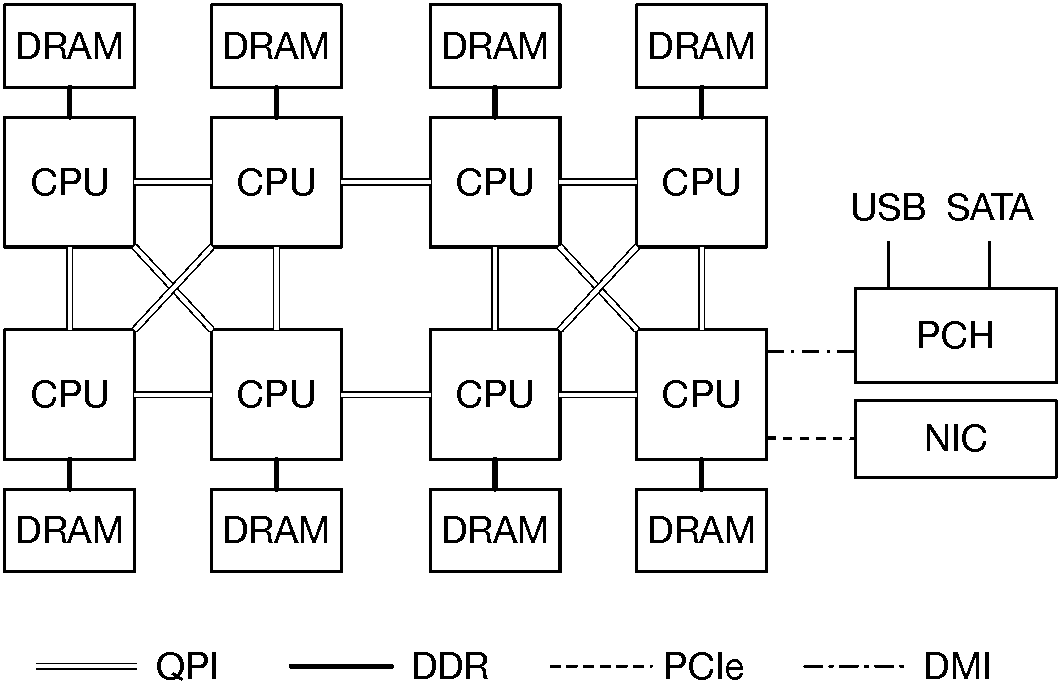
\includegraphics[width=85mm]{figures/motherboard.pdf}}
  \caption{
    The motherboard structures that are most relevant to SGX.
  }
  \label{fig:motherboard}
\end{figure}

The relevant buses are the \textit{Quick-Path Interconnect} (QPI)
\cite{intel2009qpi}, a network of point-to-point links that connect processors,
the \textit{double data rate} (DDR) bus that connects a CPU to DRAM, the
\textit {Direct Media Interface} (DMI) bus that connects a CPU to the PCH,
the \textit{Peripheral Component Interconnect Express} (PCIe) bus that connects
a CPU to peripherals such as a \textit{Network Interface Card} (NIC), and the
\textit {Serial Programming Interface} (SPI) used by the PCH to communicate
with the flash memory.

In high-end systems, the PCH also contains a service processor, called the
Intel \textit{Management Engine} (ME) \cite{ruan2014intelme}.  The ME runs
firmware stored in the same flash memory chip as the UEFI firmware. The
Management Engine is intended for remote system management and troubleshooting,
and has tremendous privileges. The ME is running even when the system is in
\textit{Soft Off} mode (ACPI G2/S5), when the CPU and RAM are unpowered. Also,
the ME can access the network via a NIC without CPU support, can read and
modify RAM via DMA transfers, and can override the CPU boot vector.

The PCIe bus is an extended, point-to-point version of the PCI standard, which
provides a method for any peripheral connected to the bus to perform
\textit{Direct Memory Access} (DMA), transferring data to and from DRAM without
involving an execution core and spending CPU cycles. The PCI standard includes
a configuration mechanism that assigns a range of DRAM to each peripheral, but
makes no provisions for preventing a rogue peripheral from accessing DRAM
outside the range that has been assigned to it.

The SGX trusted computing base includes the processor package, and excludes the
other hardware in the computer. It follows that SGX must be able to fend off
attacks from rogue devices, such as the PCIe NIC used to compromise Intel TXT
\cite{wojtczuk2011txt}, as well as passive or active bus-tapping attacks, such
as the memory bus tap used to hack the Xbox \cite{huang2003xbox} and the
memory glitching attack that subverted the PlayStation 3 hypervisor
\cite{hotz2010ps3}.

The flash memory stores the SMM handler and Intel ME firmware, which run with
high privileges. Furthermore, the contents of flash memory persists across
power cycles. This opens up the possibility for an attacker that gains SPI
access to deploy a persistent payload that runs at high privilege. To prevent
against these attacks, most of the firware is signed. For example, the ME
checks that its firmware was signed by a burned-in Intel public key. However,
both the computer firmware checks \cite{wojtczuk2010bios} and the ME firmware
checks \cite{tereshkin2009amt} have been subverted in the past.

The SGX threat model explicitly considers SMM to be untrusted. However, it does
not account for malicious code running on the Management Engine. Unfortunately,
the ME, PCH and DMI are Intel-proprietary and largely undocumented, so we
cannot assess the impact of an ME attack on software running inside an SGX
enclave.


\subsubsection{The Processor}
\label{sec:cpu_die}

An Intel processor's die, illustrated in Figure~\ref{fig:cpu_die}, is divided
into two broad areas: the \textit{core area} implements the instruction
execution pipeline typically associated with CPUs, while the \textit{uncore}
provides functions that were traditionally hosted on separate chips, but are
currently integrated on the CPU die to save power and improve latency.

\begin{figure}[hbt]
  \center{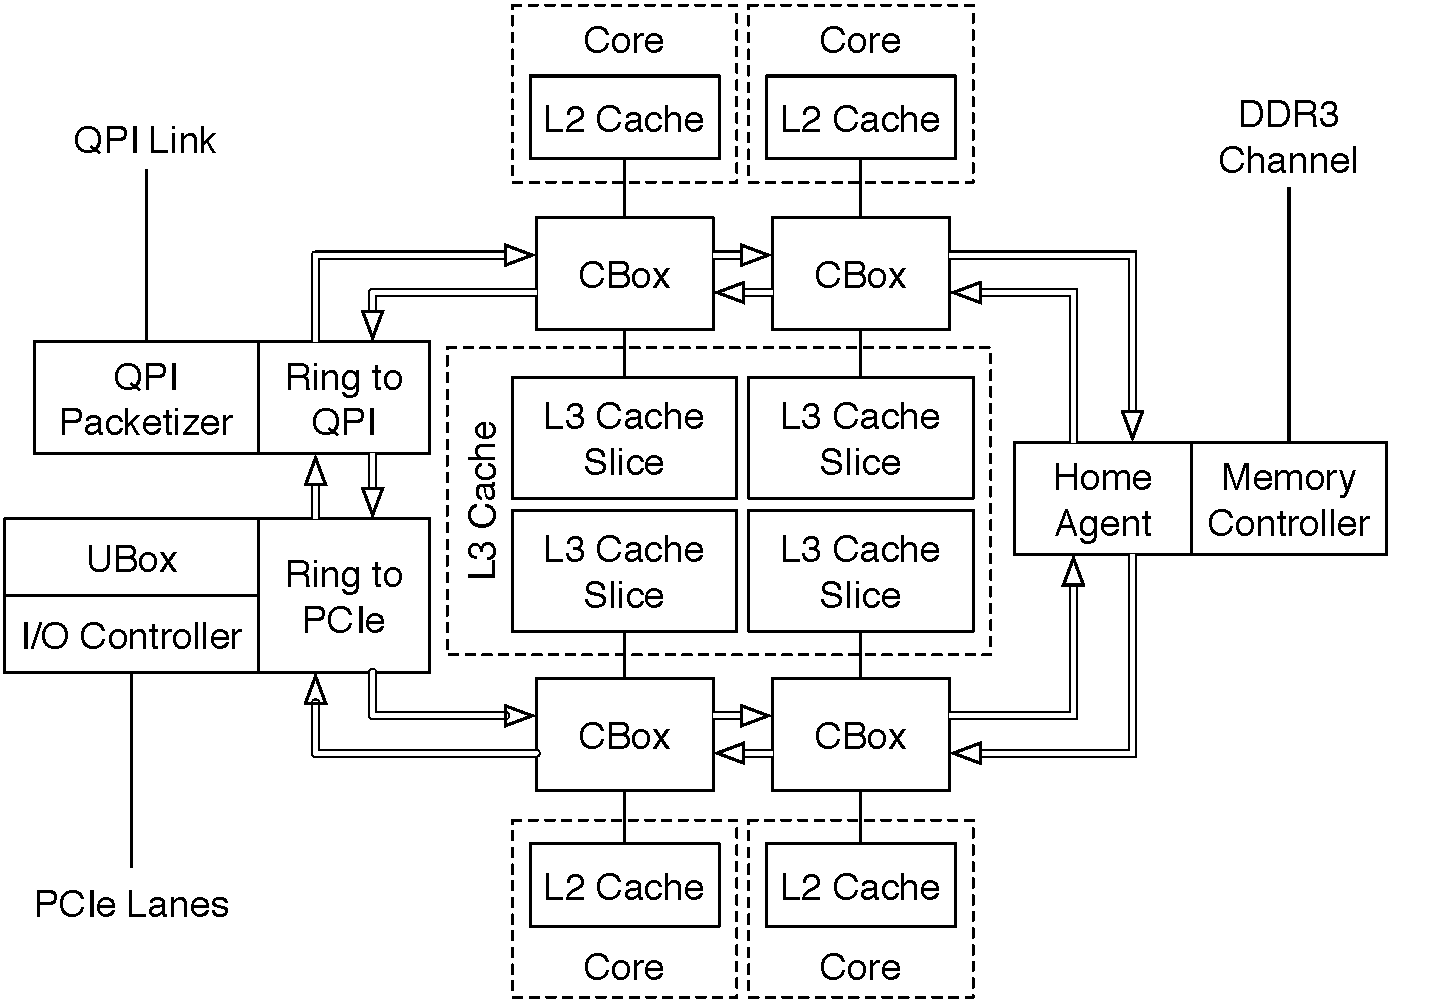
\includegraphics[width=85mm]{figures/cpu_die.pdf}}
  \caption{
    The major components in a modern CPU package. \S~\ref{sec:cpu_die} gives
    an uncore overview. \S~\ref{sec:cpu_core} describes execution cores.
    \S~\ref{sec:cache_coherence} takes a deeper look at the uncore.
  }
  \label{fig:cpu_die}
\end{figure}

% Ring Interconnect and Last Level Cache: Optimization S 2.2.5.3
% System Agent: Optimization S 2.2.6

At a conceptual level, the uncore of modern processors includes a memory
controller that interfaces with the DDR bus, an \textit{integrated I/O
controller} (IIO) that can arbitrate the PCIe bus, and a growing number of
integrated peripherals, such as a \textit{Graphics Processing Unit} (GPU), and
potentially a NIC. The uncore structure is described in some processor family
datasheets \cite{intel2014datasheet, intel2010datasheet}, and in the overview
sections in Intel's uncore performance monitoring documentation
\cite{intel2014uncore, intel2012uncore, intel2010uncore}.

The SGX design relies on the fact that the processor die includes the memory
and I/O controller, and thus can prevent any device from accessing protected
memory areas via \textit{Direct Memory Access} (DMA) transfers.
\S~\ref{sec:cache_coherence} takes a deeper look at the uncore organization and
at the mechanism used by the SGX implementation to protect sensitive memory.


\subsubsection{The Core}
\label{sec:cpu_core}

Virtually all modern Intel processors have core areas consisting of multiple
copies of the execution core circuitry, each of which is called a
\textit{core}.  At the time of this writing, desktop-class Intel CPUs have 4
cores, and server-class CPUs have as many as 18 cores.

Most Intel CPUs feature \textit{hyper-threading}, which means that a core
(shown in Figure~\ref{fig:cpu_core}) has two copies of the register files
backing the execution context described in \S~\ref{sec:registers}, and can
execute two separate streams of instructions simultaneously. Hyper-threading
increases the utilization of the shared fetch, decode and execution units, in
the presence of memory stalls.

\begin{figure}[hbt]
  \center{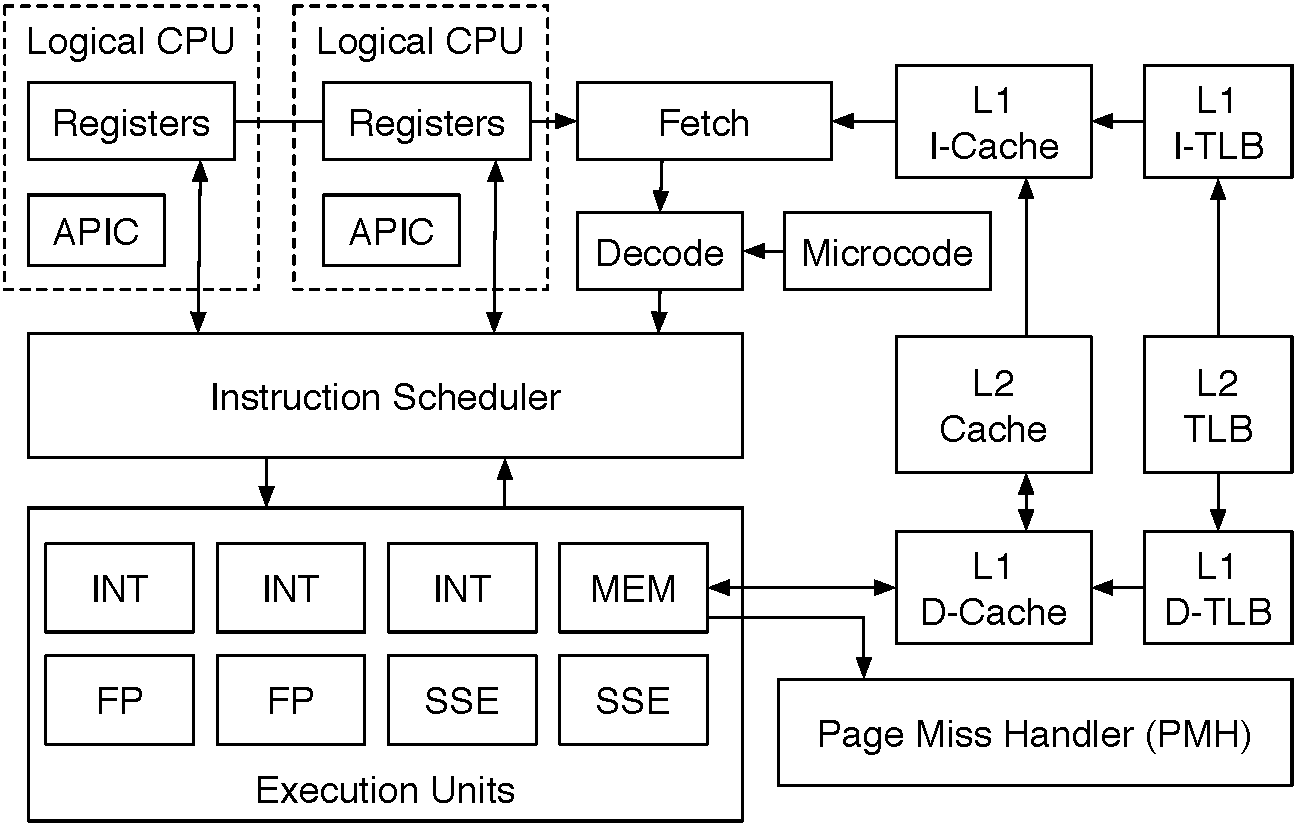
\includegraphics[width=85mm]{figures/cpu_core.pdf}}
  \caption{
    CPU core with two logical processors. Each logical processor has its own
    execution context and local APIC, and they share all the other core
    resources.
  }
  \label{fig:cpu_core}
\end{figure}

A hyper-threaded core is exposed to system software as two \textit{logical
processors}, also named \textit{hardware threads} in the Intel documentation.
The logical processor abstraction allows the code used to distribute work
across processors in a multi-processor system to function without any change on
multi-core hyper-threaded processors.

The high level of resource sharing introduced by hyper-threading introduces a
security vulnerability. Software running on one logical processor can use the
high-performance counter \cite{petters1999making} to get information about the
instructions and memory access patterns of another piece of software that is
executed on the other logical processor in the same core.
